\section{Analog-to-Digital Converter}
\subsection{Teori}
Outputtet fra målinger foretaget på biologiske signaler fremstår som et analogt signal, hvilket er kontinuert i tid og amplitude. For at kunne behandle signalet på en computer, skal signalet konverteres fra analog til digital. Det analoge signal kvantificeres under konverteringen, hvilket gør at det digitale signal bliver diskret i tid og amplitude. \citep{adc1998} Dette er illusteret på \autoref{ADC_kon}. Konverteringsprocessen består af sampling og kvantificering \citep{adc2003}. 

\begin{figure}[H]
\centering
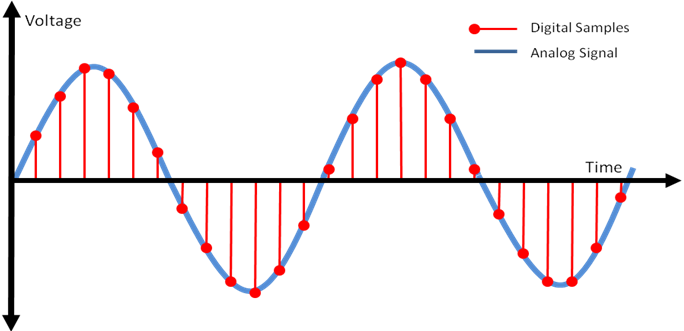
\includegraphics[width=0.6\textwidth]{figures/problemloesning/adc.png}
\caption{ADC-konvertering fra analogt til digitalt}
\label{fig:ADC_kon}
\end{figure}

Samplingsprocessen sker ved diskretisering i tidsdomænet, hvor det kontinuerte signal konverteres til et diskret signal. Det er vigtigt, at vælge en passende samplingsfrekvens for, at undgå at information fra det oprindelige signal vil gå tabt.\citep{adc2003} Ved for høj samplingsfrekvens vil en større mængde data opsamles og derved benytte mere plads og processering, hvilket vil kunne resultere i datadøden \citep{adc2004}. En for lav samplingsfrekvens vil  derimod kunne rekonstruere signalet så kurven ligger forskudt i forhold til det oprindelige signal, hvilket fremgår som alias \citep{adc2003}. I følge Nyquists sætning er det hensigtsmæssigt at samplingsfrekvens er mindst det dobbelte af frekvensen i det oprindelige signal \citep{adc2003}. I praksis anbefaldes det dog at der samples med det ti dobbelte.

Kvantificering sker ved diskretisering af amplituden. Det oprindelige signals amplitudeværdier inddeles ved kvantificering i trin. Værdierne mellem to trin repræsenteres af den samme digitale værdi, hvilket kan gøre at flere værdier ligger indenfor den samme digitale værdi \citep{adc2003}. Amplitudeniveauer der er tilgængelige til at repræsentere det analoge signal, determineres af antal bits. En ADC med en opløsning på 12-bit inddeles i {2}^{12}, svarende til 4096 niveauer. Den mindste amplitudeniveau som ADC'en kan opnå kaldes Least Significant Bit (LSB) og bestemmes ud fra ligning \autoref{equ:LSB}, hvor FSR står for Full Scale voltage Range og n antal bits. \citep{adc1998, adc2004}

\begin{equation} \label{equ:LSB}
LSB = \dfrac{\dfrac{FSR}{{2}^{12}}} 
\end{equation}

Det er vigtigt at være opmærksom på ADC'ens arbejdsområde, for at undgå at signalet bliver klippet. Ved et outputsignal der har en større range end arbejdsomsrådet for ADC'en vil signalet klippes og en del af dataen gå tabt. \citep{adc1998, adc2004}



